\section{Results}\label{sec4}
\subsection{Simulation and Comparison}
\begin{figure*}[!h]
\begin{subfigure}[b]{\textwidth}
    
    \centering
    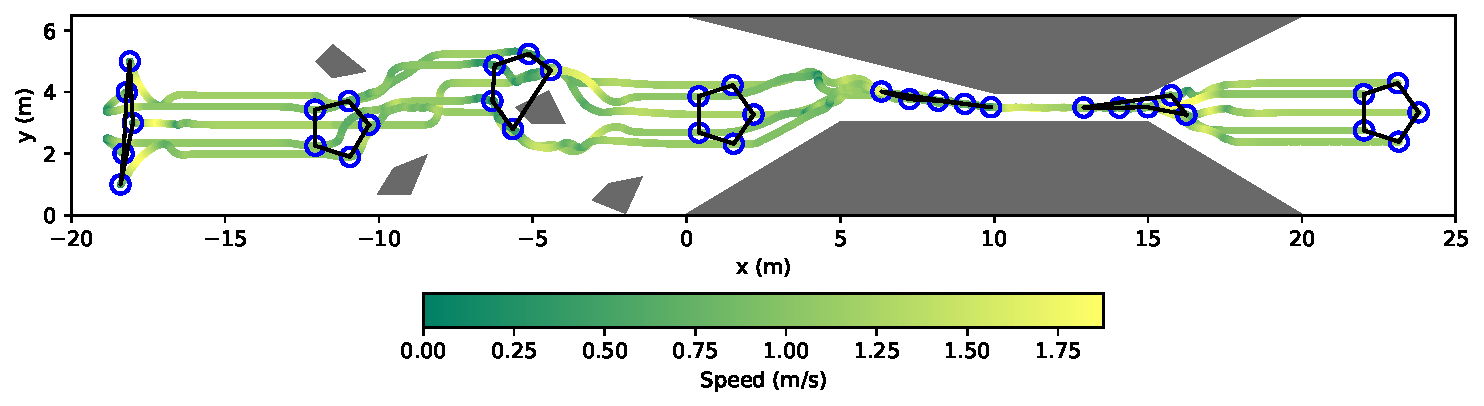
\includegraphics[width=0.9\textwidth]{paper2/images/path_edc_shape1.pdf}
    \caption{Pentagon configuration}
    \label{fig:1path_edc1}
\end{subfigure}
\begin{subfigure}[b]{\textwidth}
    \centering
    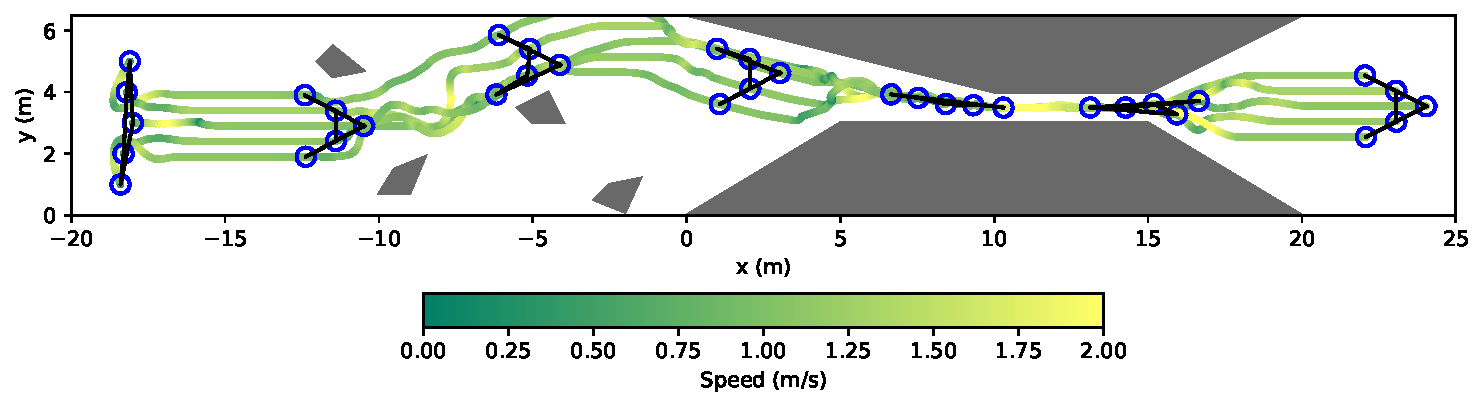
\includegraphics[width=0.9\textwidth]{paper2/images/path_edc_shape2.pdf}
    \caption{V-shape configuration}
    \label{fig:1path_edc2}
\end{subfigure}
\caption{Motion paths and velocity profiles of the proposed \textit{EDC} strategy in multiple configurations.}
\label{fig:1path}
\end{figure*}

\begin{figure*}[!h]
\begin{subfigure}[b]{0.49\textwidth}
    
    \centering
    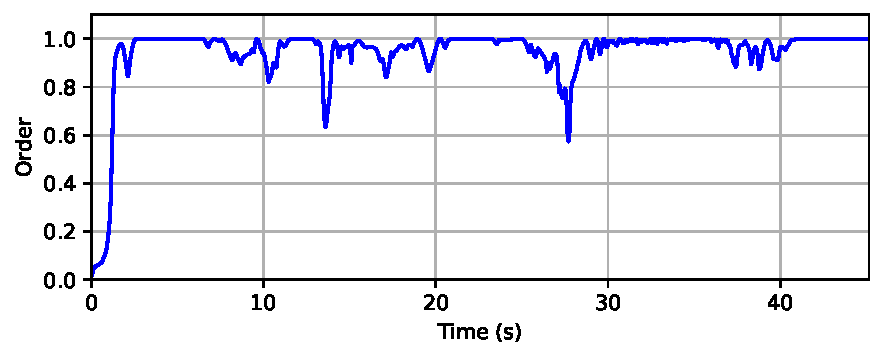
\includegraphics[width=\linewidth]{paper2/images/order_edc_shape1.pdf}
    \caption{Pentagon configuration}
    \label{fig:1order_edc1}
\end{subfigure}
\begin{subfigure}[b]{0.49\textwidth}
    \centering
    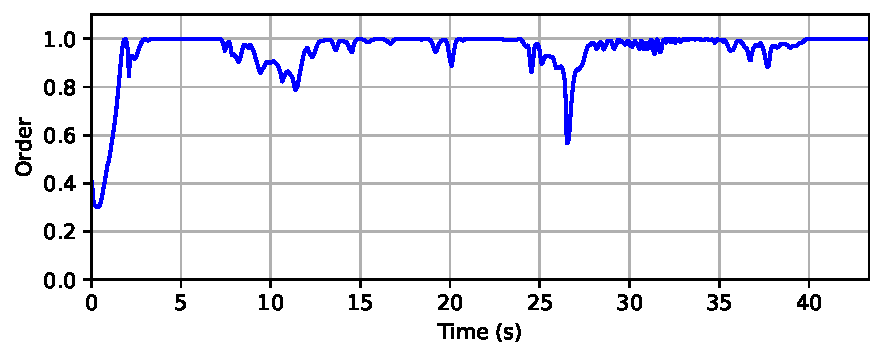
\includegraphics[width=\linewidth]{paper2/images/order_edc_shape2.pdf}
    \caption{V-shape configuration}
    \label{fig:1order_edc2}
\end{subfigure}
\caption{The \textit{order} values of the proposed \textit{EDC} strategy}
\label{fig:1order}
\end{figure*}

\begin{figure*}[!h]
\begin{subfigure}[b]{0.49\textwidth}
    
    \centering
    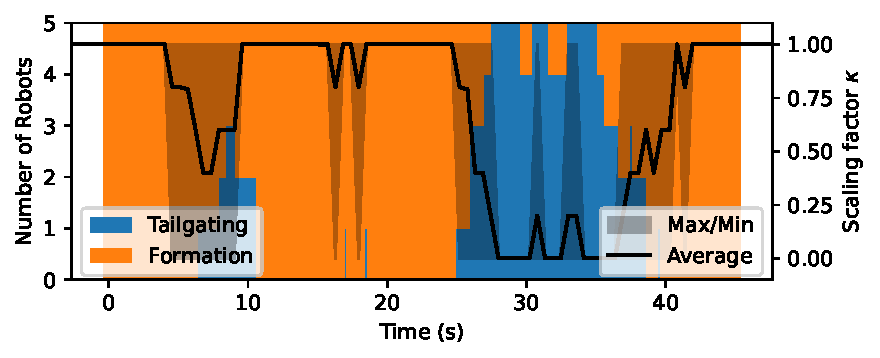
\includegraphics[width=\linewidth]{paper2/images/mode_edc_shape1.pdf}
    \caption{Pentagon configuration}
    \label{fig:1mode_edc1}
\end{subfigure}
\begin{subfigure}[b]{0.49\textwidth}
    \centering
    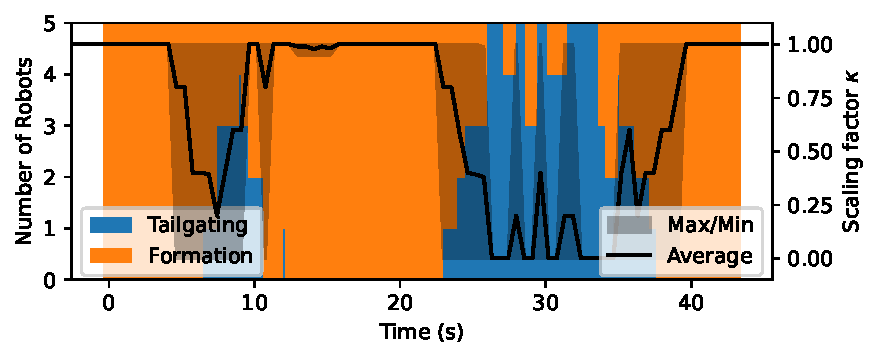
\includegraphics[width=\linewidth]{paper2/images/mode_edc_shape2.pdf}
    \caption{V-shape configuration}
    \label{fig:1mode_edc2}
\end{subfigure}
\caption{Correlation of number of robots and scaling factor of the proposed \textit{EDC} strategy}
\label{fig:1mode}
\end{figure*}

% The simulations are run on AMD Ryzen 5 5500U with a base frequency of 2.1 GHz. 
The proposed strategy is tested in a complex environment, which consists of 2 areas of different obstacle types, one area is the forest-liked environment, whose obstacle densities is 0.05 obs/m$^2$ (for $-12$~m $<x<0$~m), another area is the width-varying cave-like environment with the most narrowed space is 1~m (for $0$~m $<x<20$~m). The TVF starts randomly from the left-hand side of the environment and has a mission to travel through the confined space to the right-hand side, with the desired direction $u_\text{ref}=\left[1,0,0\right]^T$. We set up a formation with 5 homogeneous robots with two formation configurations, including V-shape and polygon configurations, when the TVF transforms to \textit{``Tailgating''} mode, the desired distance for a robot to follow its leader is set by $d_\text{ref}=1$~m. They have constraints with $v_\text{max}=2$~m/s and $u_\text{max}=2$~m/s$^2$. The control period is set at $\tau=0.1$~s. The comparison is done with pure behavior-based control (BC)~\cite{736776,Vsrhelyi2018}. For comparison between the different methods, the following performance metrics are used: success rate, mean speed, and mean acceleration cost $(\sum{\left\Vert u(k)\right\Vert^2}/{nT})$, with $T$ is the total travel time of the TVF. The parameters used in both strategies are the same to ensure fairness.

In the simulation, we examined how the \textit{EDC} guided a TVF to navigate through confined spaces. The motion paths and corresponding velocity profile are presented in Fig.~\ref{fig:1path}. Both two formations, including polygon and V-shape configurations, successfully navigate through confined spaces, which include forest-like and tunnel-like environments. Initially, all robots were on the left-hand side, which did not form the desired configuration. They move in the desired direction and form to the predefined shape. Whenever obstacles are detected, the robot activates the obstacle avoidance behavior, there is no narrow space in the first area, and robots in the formation maintain the \textit{``Formation''} mode. Once narrow space is observed, the TVF transforms to \textit{``Tailgating''} mode, which is assigned itself by each robot observation. The straight line configuration is then created, which can help the formation pass through the gap. When the robot escapes the narrow passage, the mode turns back to \textit{``Formation''} mode, which reforms to the desired configuration. Finally, the formation successfully passes through the confined space. Fig.~\ref{fig:1path} presents the motion paths of the TVF, which are conducted by the proposed strategy in multiple configurations.

To further investigate the effectiveness of the proposed strategy, the \textit{order} $\Phi$ metric is defined to measure the heading disturbance of robots in formation during movement. The order's values are in $\left[0,1\right]$, and if the formation has no heading, the order is close to 1 \cite{Vicsek1995}.
\begin{equation}
    \Phi=\dfrac{1}{n}\left\Vert\sum_{i=1}^n{\dfrac{v_i}{\left\Vert v_i\right\Vert}}\right\Vert
\end{equation}
where $v_i$ is the velocity of robot $i$.

Fig.~\ref{fig:1order} illustrates the order information of the TVF's heading throughout the movement process. The figures reveal that the heading order of the swarm in both two scenarios during movement is satisfactory ($\Phi = 1$), When the formation encounters obstacles, the \textit{order} value is changed but still forms the overall configuration. However, disorderliness in the heading order becomes apparent during the transition from \textit{``Formation''} to \textit{``Tailgating''} and vice versa. This is because the structure of the formation undergoes a significant change, resulting in a disorderly heading order.

Fig~\ref{fig:1mode} describes the correlation between the number of robots in different modes and the scaling factor $\kappa$ to evaluate the effectiveness of the synthesized controllers in the proposed deformation strategy. When the TVF encounters obstacles, the configuration is adapted based on the observation of each robot. As a result, the mode of each robot is different at the same time. Also, the scaling factor $\kappa$ is different between robots in the TVF, due to its position and the observation. In collision-free, all robots in the TVF remain in \textit{``Formation''} mode, which contributes to maintaining the original configuration. On the other hand, when narrow space is detected by all robots, the mode transforms to \textit{``Tailgating''}, which forces robots to the straight line configuration to safely navigate through narrow space. The value of $\kappa=0$ when all robots in the TVF are in the \textit{``Tailgating''} mode.

\begin{table}
\caption{Comparison between \textit{BC} and our method, \textit{EDC}. Each comparison is over 10 simulations of 5 robots in two different configurations. The metrics displayed in the table are the success rate, mean speed, and mean acceleration cost.}
\label{tbl:com}
\centering
\begin{tabular}{C{3.2cm} C{2.cm} C{2.0cm} C{3.0cm} C{3.0cm}}
\hline\hline
Configuration             & Strategy & Succ. & Mean speed (m/s) & Mean Acc. cost (m$^2$/s$^4$)  \\ \hline
\multirow{2}{*}{Pentagon} & EDC      & \textbf{10/10}        & 0.6773   & \textbf{3.6873}          \\
                          & BC       & 0/10    & \textbf{0.7785}   & 4.3874      
                          \\ \hline
\multirow{2}{*}{V-shape}  & EDC      & \textbf{10/10}        & 0.7129   & \textbf{4.0978}          \\
                          & BC       & 0/10   & \textbf{0.8877}      & 4.9402 \\ \hline\hline    
\end{tabular}
\end{table}

To further verify the effectiveness of the proposed strategy against the pure behavioural-based control (BC)~\cite{736776,Vsrhelyi2018}, Table~\ref{tbl:com} presents a comparison between proposed strategy, \textit{EDC} and BC. It can be seen that the proposed \textit{EDC} strategy outperforms the \textit{BC} in success rate, which can navigate formation passes through a confined space without any collision. Meanwhile, the \textit{BC} always fails when encountering a narrow space (see Fig.~\ref{fig:1sample}). The mean acceleration cost per time is also smaller than the \textit{BC}, because \textit{BC} costs more energy to deal with the surrounding obstacles. The \textit{EDC} provides an effective method to deal with obstacles by the adaptation configuration. However, the mean speed of the TVF is slightly smaller than the standard approach, due to the translation mode while moving affect to the speed down of the TVF.

\subsection{Validation on the software-in-the-loop Gazebo}
\begin{figure*}[h!]
    \centering
    \begin{subfigure}[b]{0.45\textwidth}
    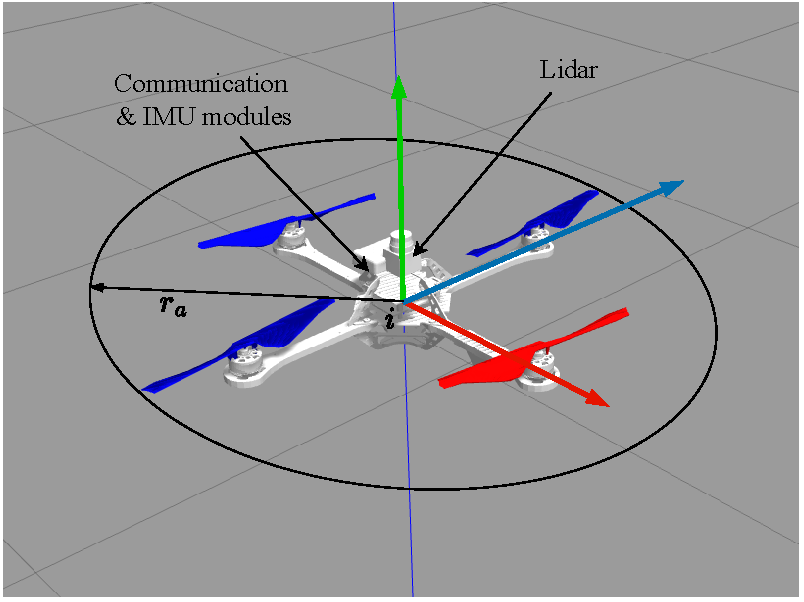
\includegraphics[width=\textwidth]{paper2/images/gazebo_uav.pdf}
    \caption{Gazebo SIL model}
    \label{fig:1gazebo_uav}
    \end{subfigure}
    \begin{subfigure}[b]{0.44\textwidth}
    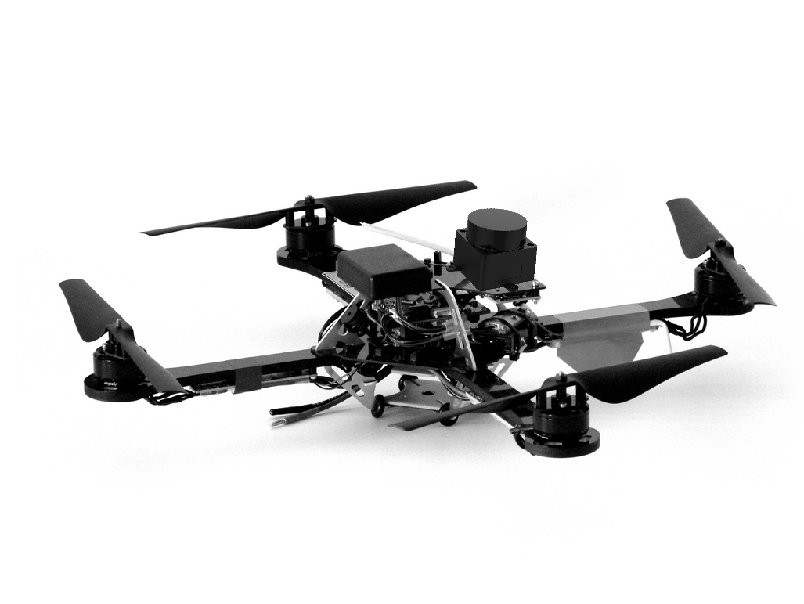
\includegraphics[width=\textwidth]{paper2/images/hummingbird.pdf}
    \caption{Real UAV model \cite{Furrer2016,Bui2022}}
    \label{fig:1gazebo_real}
    \end{subfigure}
    \caption{Used Hummingbird UAV model}
    \label{fig:1gazebo_setup}
\end{figure*}

\begin{figure*}[h!]
    \centering
    \begin{subfigure}[b]{0.495\textwidth}
    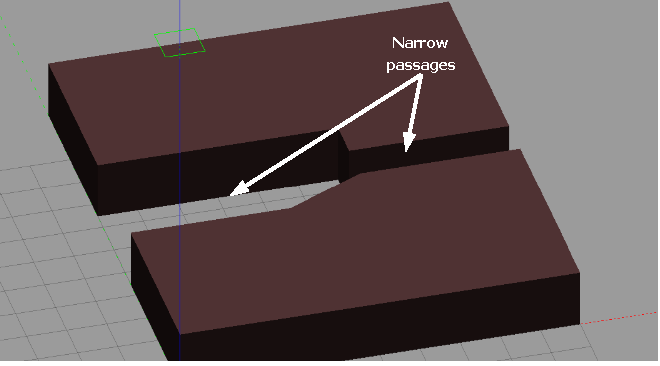
\includegraphics[width=\textwidth]{paper2/images/gazebo_env.pdf}
    \caption{The Gazebo environment}
    \end{subfigure}
    \begin{subfigure}[b]{0.40\textwidth}
    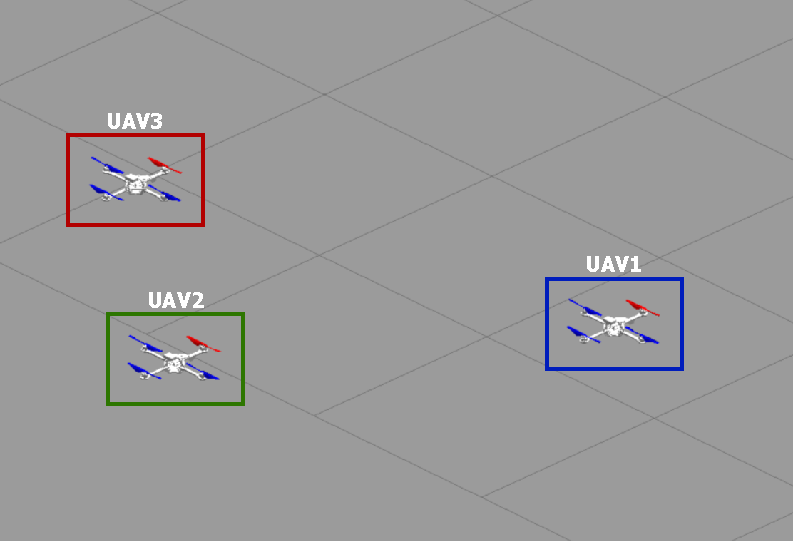
\includegraphics[width=\textwidth]{paper2/images/gazebo_init.pdf}
    \caption{Random initial positions}
    \label{fig:1gazebo_init}
    \end{subfigure}
    \caption{The environment in SIL test}
    \label{fig:1gazebo_env}
\end{figure*}

\begin{figure*}
    \centering
    \begin{subfigure}[b]{0.48\textwidth}
    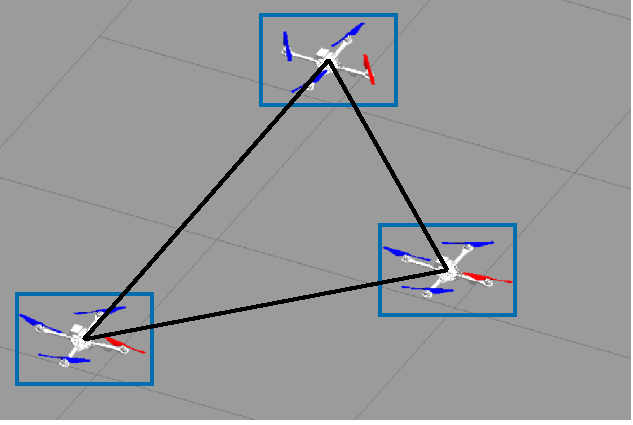
\includegraphics[width=\textwidth]{paper2/images/gazebo_res1.pdf}
    \caption{Maintain triangle formation from random}
    \label{fig:1gazebo_1}
    \end{subfigure}
    \begin{subfigure}[b]{0.48\textwidth}
    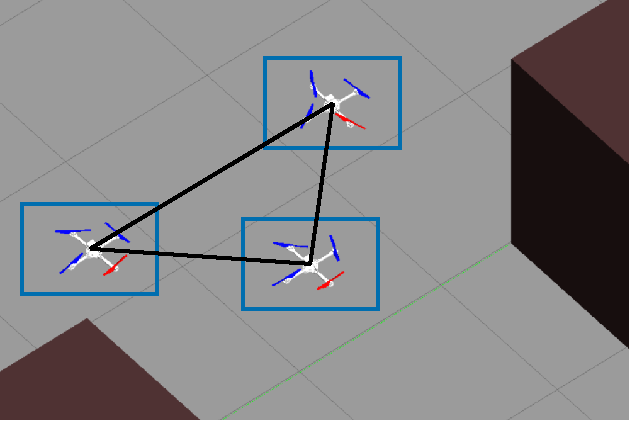
\includegraphics[width=\textwidth]{paper2/images/gazebo_res2.pdf}
    \caption{Small-scaled triangle formation}
    \label{fig:1gazebo_2}
    \end{subfigure}
    \begin{subfigure}[b]{0.48\textwidth}
    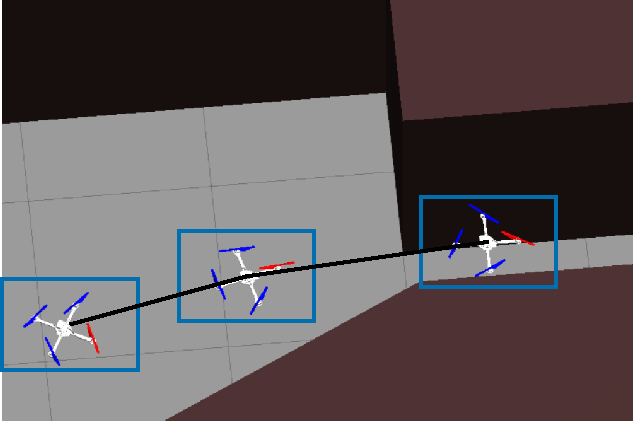
\includegraphics[width=\textwidth]{paper2/images/gazebo_res3.pdf}
    \caption{Transform to line formation}
    \label{fig:1gazebo_3}
    \end{subfigure}
    \begin{subfigure}[b]{0.48\textwidth}
    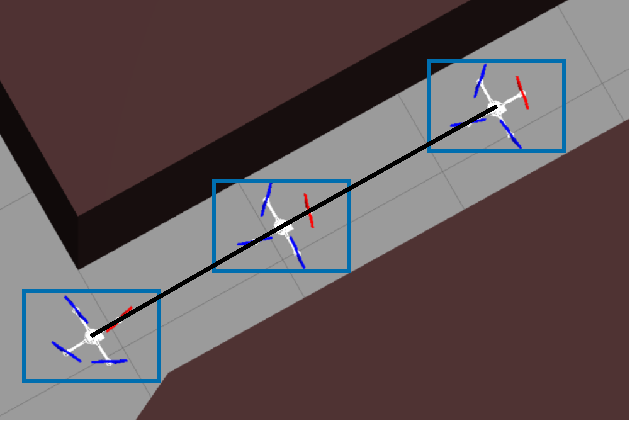
\includegraphics[width=\textwidth]{paper2/images/gazebo_res4.pdf}
    \caption{Line formation}
    \label{fig:1gazebo_4}
    \end{subfigure}
    \begin{subfigure}[b]{0.48\textwidth}
    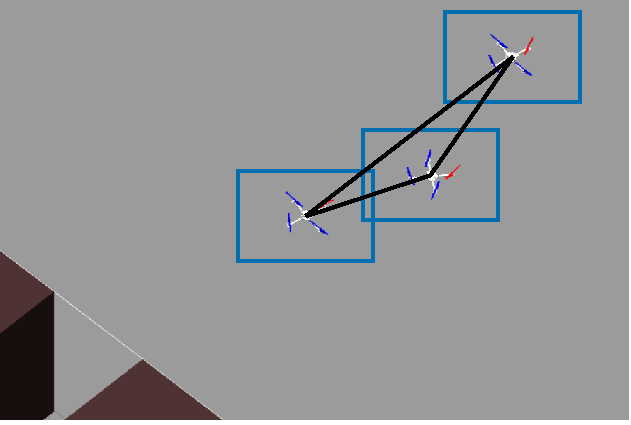
\includegraphics[width=\textwidth]{paper2/images/gazebo_res5.pdf}
    \caption{Transform back to triangle formation}
    \label{fig:1gazebo_5}
    \end{subfigure}
    \begin{subfigure}[b]{0.48\textwidth}
    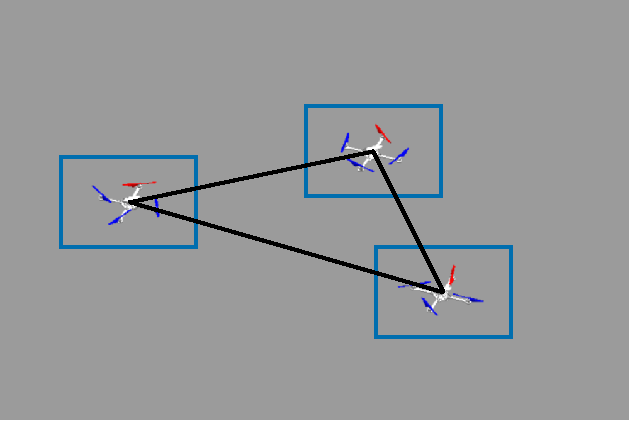
\includegraphics[width=\textwidth]{paper2/images/gazebo_res6.pdf}
    \caption{Original triangle formation}
    \label{fig:1gazebo_6}
    \end{subfigure}
    \caption{Validation results captured in the SIL Gazebo}
    \label{fig:1gazebo_result}
\end{figure*}

\begin{figure*}
    \centering
    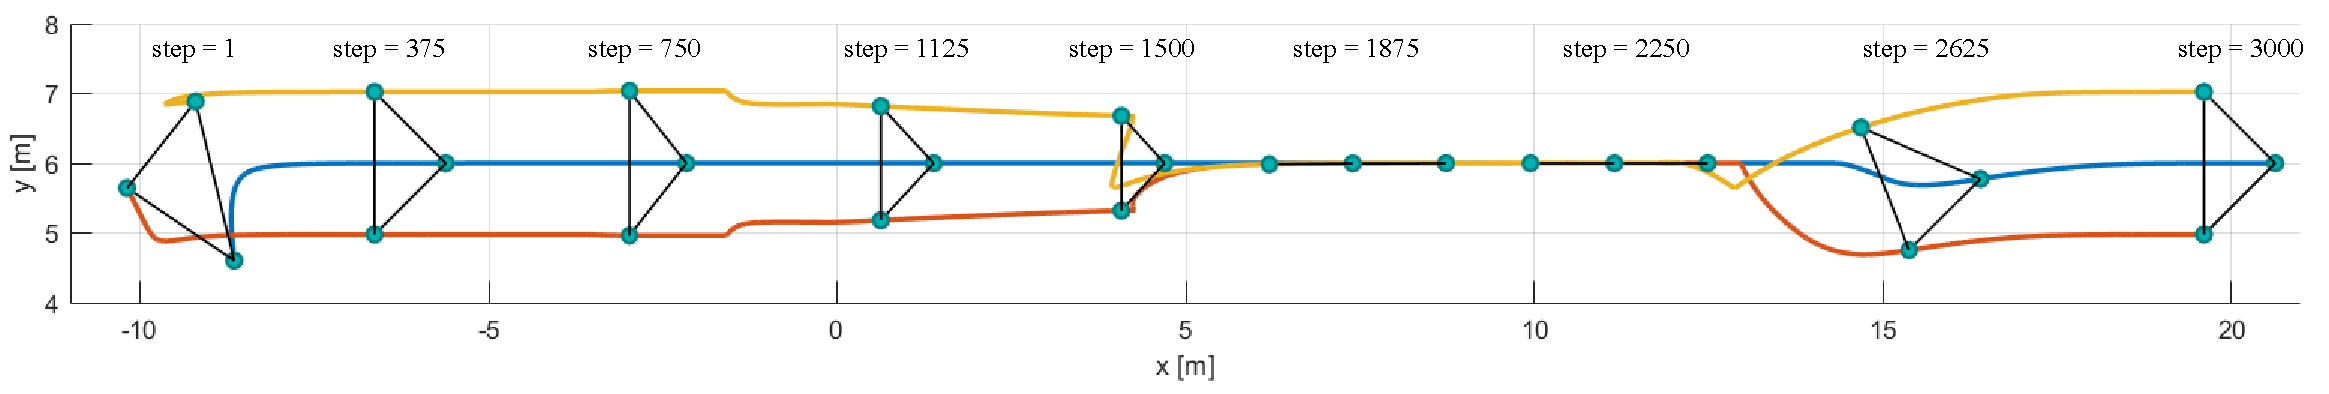
\includegraphics[width=\textwidth]{paper2/images/gazebo_path.pdf}
    \caption{The recorded paths of three UAV in the SIL test (Top view)}
    \label{fig:1gazebo_path}
\end{figure*}

To evaluate the applicability of the proposed system, we have conducted a software-in-the-loop (SIL) validation that involves navigating UAV formation pass through a confined space, which only focuses on a narrow tunnel-like environment in a Gazebo\footnote{Gazebo experiment video: {\fontfamily{qcr}\selectfont
\url{https://youtu.be/AIAAzRiIepg}}}. The used UAV model is a Hummingbird quadrotor developed based on Gazebo-based RotorS simulator~\cite{Furrer2016}, as described in Fig.~\ref{fig:1gazebo_uav}. We set up three UAVs in the experiment with random positions, as shown in Fig.~\ref{fig:1gazebo_init}. The environment in the SIL test includes two large obstacles, forming a width-varying tunnel, as depicted in Figure \ref{fig:1gazebo_env}.

Fig.~\ref{fig:1gazebo_result} presented the formation moving captured in the experiment. Moreover, the paths of three UAVs in the SIL test are recorded and are depicted in Fig.~\ref{fig:1gazebo_path}. At the beginning of the motion (step 1), three UAVs are in the random position. They then move to form the desired triangle formation (steps 375 - 750), as shown in Fig.~\ref{fig:1gazebo_1}. When sensing the narrow passage, the formation shrinks to safely move through the passage (steps 1125 - 1500), as shown in Fig.~\ref{fig:1gazebo_2}. When the narrow space is not suitable for the original formation, the formation transforms to the straight line formation as Fig.~\ref{fig:1gazebo_3} and then passes through the space with the line formation (steps 1875 - 2550), as Fig.~\ref{fig:1gazebo_4}. Once the UAV senses enough space in the environment to maintain its original formation, the formation transforms back to the origin shape in Fig.~\ref{fig:1gazebo_5} and moves to the target in Fig.~\ref{fig:1gazebo_6} (steps 2625 - 3000). The experiment demonstrates that the proposed \textit{EDC} strategy successfully navigates the UAVs' formation to the target by passing through the narrow passage.

% \subsection{Discussion}
% Through simulation, validation, comparative statistics, and SIL testing, it is clear that our proposed method is capable of navigating the formation ensuring configuration, safety, and optimality for robot operation in narrow space environment.

% The proposed strategy provides flexibility for the robot formation to move safely through narrow space environments with numerous of formation configuration the ability to scale, rotate, and transform into a line configuration based on the perception of the environment depicted in Figure \ref{fig:1path}.

% The proposed algorithm also ensures scalability across various robot quantities within the formation, as presented in Figure \ref{fig:1path}. As long as the robots adhere to the specified configuration, the strategy offers the flexibility to navigate through narrow environments effectively.

% In our design, the formation maintenance and tailgating behaviors are proven to be stable through Lyapunov's theorem (see Appendix \ref{app:uf} and Appendix \ref{app:ut}), which proves that the system errors will converge to zero, as provided in Figure \ref{fig:1error}. Their convergence speed can be controlled through the parameters, $k_f$, $k_t$.

% On another note, our proposed strategy brings forth the capability to swiftly respond to environmental variations and traverse narrow spaces securely. Nonetheless, the transitions between states and abrupt alterations in formation size may result in occasional movement disruptions (see \textit{order} metric in Figure \ref{fig:1metric}). In such instances, employing control techniques like fuzzy logic or neural networks can be employed to improve the overall fluidity of formation movement.